\chapter{Transporte Óptimo de Masas}
\label{chap:transporte-optimo-de-masas}

En este capítulo se abordará el problema de transporte óptimo, la distancia de Wasserstein, y el problema de los baricentros de Wasserstein. Además, se presentarán algunas propiedades de la distancia de Wasserstein que serán de utilidad en el desarrollo de este trabajo. La notación, definiciones y explicaciones utilizadas están basadas principalmente en \cite{villani2009optimal}, \cite{peyre2019computational} y \cite{panaretos2020invitation}.

\section{Notación}
 {
  \FM[inline]{Agregar alguna intro para lo que es una medida de probabilidad? para aquellas personas que vienen de otras áreas?}
  \begin{definition}
	  \FM[inline]{Se podría dejar notación probabilística?}
	  Se definen los siguientes espacios:
	  \begin{itemize}
		  \item $(\cX, \dist)$ es un espacio Polaco, si $\cX$ es un espacio métrico, completo y separable.
		  \item $\ProbSpace[\cX]$ denotará al conjunto de medidas de probabilidad en $\cX$, utilizando la $\sigma$-álgebra de Borel.
		  \item $\ProbSpaceAC[\cX]$ denotará al conjunto de medidas de probabilidad absolutamente continuas con respecto a una medida de referencia $\lambda$ (como por ejemplo, la de Lebesgue o la cuenta puntos), utilizando la $\sigma$-álgebra de Borel.
		  \item $\mathcal{C}(\cX)$ denotará al conjunto de funciones continuas en $\cX$.
		  \item ${\Lip}_{k}(\cX)$ denotará al conjunto de funciones $k$-Lipschitz en $\cX$. Mientras que se asumirá que $\Lip[\cX]$ denotará al conjunto de funciones $1$-Lipschitz en $\cX$. \FM[inline]{Se podría agregar una definición de función Lipschitz?}
	  \end{itemize}
  \end{definition}

  %   \begin{definition}
  % 	  Se definirá el \emph{simplex} de dimension $n$ como el conjunto de vectores de $\R^{n}$ cuyas componentes suman 1, es decir,
  % 	  \begin{equation}
  % 		  \Simplex \eqdef \left\{
  % 		  x \in [0, 1]^{n} \colon \sum_{i=1}^{n} x_{i} = 1
  % 		  \right\},
  % 	  \end{equation}
  % 	  y a los elementos pertenecientes al simplex se les llamará \emph{vectores de probabilidad}.
  %   \end{definition}


 }

\section{El Problema de Transporte}
 {
  A lo largo de esta sección, se presentarán distintas formulaciones del problema de transporte, comenzando con sus orígenes \cite{monge1781memoire}, seguido de su formulación relajada \cite{kantorovich1942translocation}, y concluyendo al destacar que, en realidad, ambos problemas son dos caras de una misma moneda \cite{brenier1991polar}. Es notable señalar que muchos ejemplos han sido tomados e inspirados de \cite{panaretos2020invitation}, \cite{peyre2019computational} y \cite{cuturi2017primer}.

  %   A lo largo de esta sección se presentarán distintas formulaciones de lo que es el problema de transporte, empezando con sus orígenes \cite{monge1781memoire}, pasando con su formulación relajada \cite{kantorovich1942translocation}, y finalizando comentando que, realmente, ambos problemas son dos caras de una misma moneda \cite{brenier1991polar}. Cabe destacar que muchos ejemplos en esta sección han sido tomados e inspirados de \cite{panaretos2020invitation}, \cite{peyre2019computational} y \cite{cuturi2017primer}.

  \subsection*{El problema de Monge}
  {

	  %   En esta sección, se tomará la introducción realizada en el libro \emph{An Invitation to Statistics in Wasserstein Space}, de \cite{panaretos2020invitation}.

	  Supongamos que hay un trabajador que debe de transportar una pila de arena a un pozo de igual volumen, situación que se puede ver representada en la Figura~\ref{fig:montanas-arena-pozo}. Dada esta situación, \cite{monge1781memoire} se preguntó: ¿Cuál es la manera de transportar la arena al pozo con \emph{el menor esfuerzo} para el trabajador?, o dicho de otra manera, ¿Cuál es la forma \emph{óptima} de transportar la arena al pozo?

	  %   \cite{monge1781memoire} un día se preguntó: dada una pila de arena y un pozo de igual volumen como en la Figura~\ref{fig:montanas-arena-pozo}, ¿Cuál es la forma óptima de transportar la arena al pozo? o dicho de otra manera, ¿Cuál es la manera de transportar la arena al pozo con el menor esfuerzo?

	  \begin{figure}[ht]
		  \centering
		  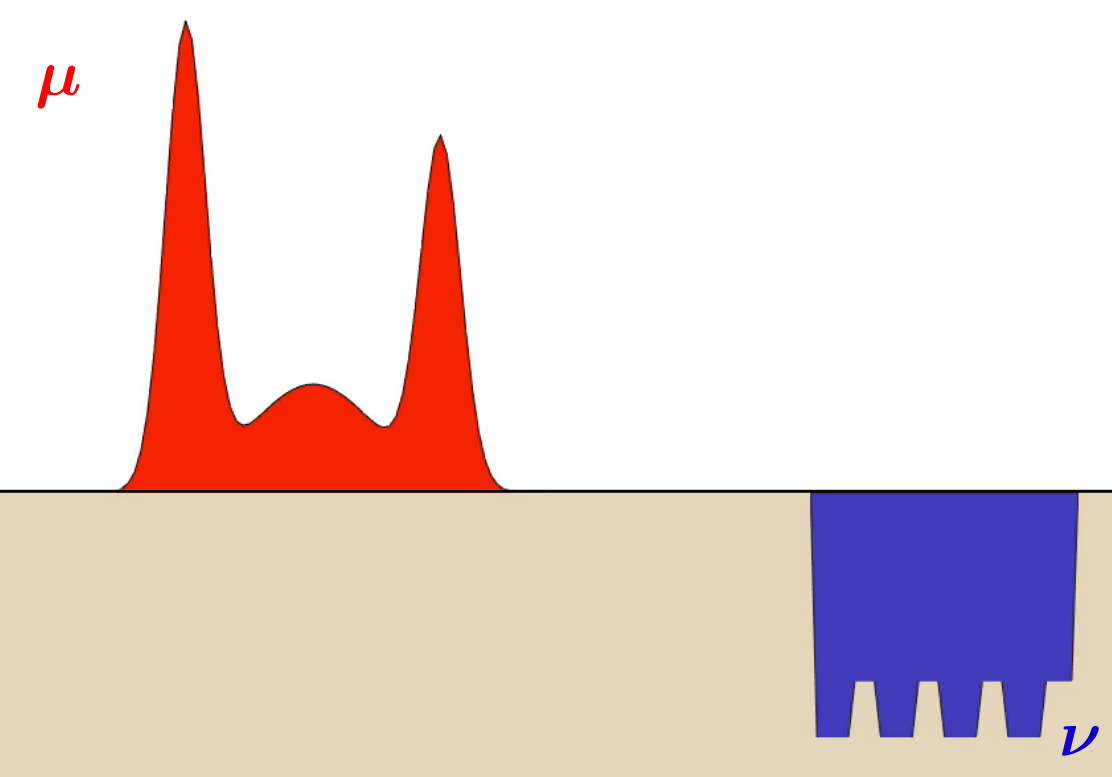
\includegraphics[width=0.5\textwidth]{img/transporte/montanas-arena-pozo.png}
		  \caption{Representación de la pila de arena, representada en rojo por la medida $\mu$, y el pozo, representada en azul por la medida $\nu$. Imagen obtenida de \cite{cuturi2017primer}.}
		  \label{fig:montanas-arena-pozo}
	  \end{figure}

	  Utilizando términos matemáticos, este problema se formula de la siguiente manera: dado un espacio de arena $\cX$, un espacio de pozo $\cY$, y una función de costo $c: \cX \times \cY \to \R$, que representa el esfuerzo necesario para transportar una unidad de arena del punto $x \in \cX$ a una posición en el pozo $y \in \cY$. La distribución de la arena se describe mediante una medida $\mu \in \ProbSpace[\cX]$, mientras que la forma del pozo se caracteriza mediante una medida $\nu \in \ProbSpace[\cY]$.

	  La \emph{decisión} sobre cómo transportar la arena se representa mediante una función $T: \cX \to \cY$, que asigna a cada punto $x \in \cX$ una posición $T(x) \in \cY$ en el pozo. El ``esfuerzo total'' que el trabajador debe realizar corresponde a ``sumar'' el costo asociado al transporte de la arena desde $x$ hasta la posición correspondiente en el pozo $T(x)$. Más formalmente, el \emph{costo total} de transportar la arena al pozo se obtiene integrando el costo mencionado anteriormente sobre todo el espacio de arena:
	  \begin{equation}\label{eq:costoTotalTransporteMonge}
		  C(T) \eqdef \int_{\cX} c(x, T(x)) \dmu[x].
	  \end{equation}

	  \begin{figure}[ht]
		  \centering
		  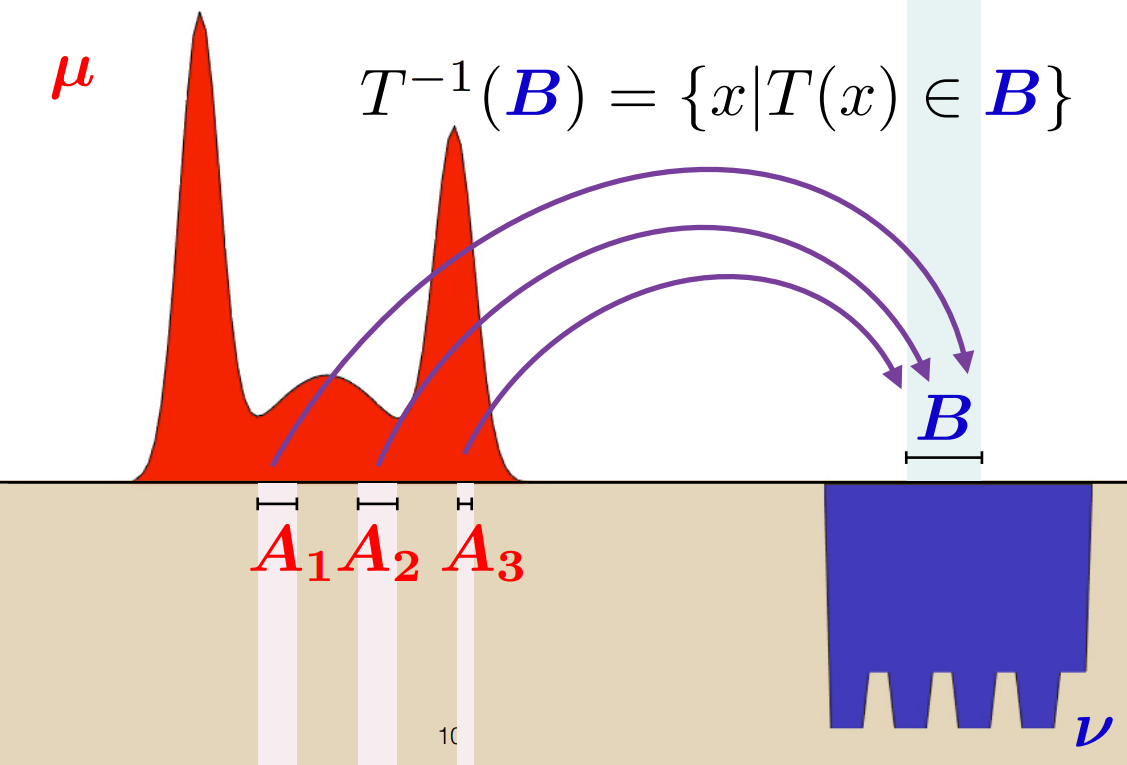
\includegraphics[width=0.5\textwidth]{img/transporte/preservacion-masa.png}
		  \caption{Representación de como la función $T$ ha de preservar la masa total de la arena. Imagen obtenida de \cite{cuturi2017primer}.}
		  \label{fig:preservacion-masa}
	  \end{figure}

	  Una primera propiedad que se debe exigir a la función $T$ es que preserve la masa total de la arena. Es decir, para cualquier conjunto $B \subseteq \cY$ que represente una región en el pozo con volumen $\nu(B)$, se requiere que el volumen de arena asignado a la región $B$ por la ``decisión'' $T$ sea exactamente el mismo volumen que se rellenará en $B$. La cantidad de arena que ocupará $B$ bajo la ``decisión'' $T$ se expresa como $\left\{ x \in \cX : T(x) \in B \right\} = T^{-1}(B)$, y por lo tanto, la condición de preservación de masa implica que $\mu(T^{-1}(B)) = \nu(B)$ para todo $B \subseteq \cY$.

	  Esta condición se ilustra gráficamente en la Figura~\ref{fig:preservacion-masa} y se formula de manera más precisa mediante la siguiente definición:

	  \begin{definition}[Operador push-forward]
		  Sea una función medible $T:\cX \to \cY$, se define el \emph{operador push-forward}  de $T$ como la aplicación $\Tpf:\ProbSpace[\cX] \to \ProbSpace[\cY]$ que satisface la siguiente relación:
		  \begin{equation}
			  \label{eq:pushForward}
			  \Tpf \mu(B) \eqdef \mu (T^{-1}(B)) = \nu(B),\quad \forall B \subseteq \cY \text{ medible}.
		  \end{equation}
	  \end{definition}

	  Ahora que disponemos de todas las herramientas matemáticas necesarias, podemos definir este problema como el de encontrar una función $T$ que representa la manera de transportar la arena al pozo, tal que minimice el ``esfuerzo'' de transporte $C(T)$, sujeto a la condición de que la masa total de la arena sea preservada. De manera más formal:

	  \begin{definition}[Problema de \cite{monge1781memoire}]
		  Dadas dos medidas $\mu \in \ProbSpace[\cX]$ y $\nu \in \ProbSpace[\cY]$ y una función de coste $c : \cX \times \cY \to \R$, el \emph{problema de transporte óptimo de Monge} se define como el problema de encontrar una función medible $T: \cX \to \cY$ que minimice el costo total de transporte $C(T)$. Es decir, que minimice la siguiente expresión:
		  \begin{equation}
			  \label{eq:problemaTransporteMonge}
			  \inf_{T: \Tpf \mu = \nu} \int_{\cX} c(x, T(x)) \dmu[x].
		  \end{equation}
		  A aquella función $T$ que resuelva este problema se le llamará \emph{función de transporte} o \emph{mapa de transporte}, y se denotará por $T_{\mu \to \nu}$, o simplemente $T$ si es que no existe confusión.
	  \end{definition}

	  El problema introducido por \cite{monge1781memoire} es, en general, considerablemente difícil. Esto se debe principalmente a que el conjunto de mapas de transporte $\left\{ T : \Tpf \mu = \nu \right\}$ es intratable. Además, puede suceder que no exista ninguna solución, o en el caso de que exista, esta podría no ser única, como veremos en los siguientes ejemplos:

	  \begin{example}\label{ex:problemaDeMongeSinSolucion}
		  Consideremos $\cX = \left\{ -1, 1 \right\}$, $\cY = \left\{ 0 \right\}$, con $\mu = \frac{1}{2} \delta_{-1} + \frac{1}{2} \delta_{1}$ y $\nu = \delta_0$. En este caso, la función de transporte óptima que minimiza \eqref{eq:problemaTransporteMonge} es
		  \begin{align*}
			  T_{\mu \to \nu}(-1) & = 0 & T_{\mu \to \nu}(1) & = 0.
		  \end{align*}
		  Sin embargo, es importante destacar que no existe un transporte óptimo $T_{\nu \to \mu}$ que transporte la masa de $\nu$ a $\mu$. Esto se debe a que la masa de $\nu$ está concentrada en un solo punto, mientras que la masa de $\mu$ está distribuida en dos puntos. No es posible ``dividir'' la masa debido a la naturaleza determinista de los mapas de transporte. Este ejemplo ilustra un caso en el que el problema de Monge no tiene solución.
	  \end{example}

	  \begin{example}\label{ex:problemaDeMongeMultipleSolucion}
		  Consideremos ahora $\cX = \left\{ (1, 1), (-1, -1) \right\}$, $\cY = \left\{ (-1, 1), (1, -1) \right\}$, con $\mu = \frac{1}{2} \delta_{(1, 1)} + \frac{1}{2} \delta_{(-1, -1)}$ y $\nu = \frac{1}{2} \delta_{(-1, 1)} + \frac{1}{2} \delta_{(1, -1)}$. Este ejemplo correspondería a uno en que los puntos de $\cX$ y $\cY$ forman un cuadrado. En este escenario, se observa que existen dos funciones de transporte óptimo $T^1_{\mu\to\nu}$ y $T^2_{\mu\to\nu}$ que minimizan \eqref{eq:problemaTransporteMonge}. Estas funciones se expresan como:
		  \begin{align*}
			  T^1_{\mu\to\nu}(1, 1) & = (1, -1) & T^1_{\mu\to\nu}(-1, -1) & = (-1, 1)  \\
			  T^2_{\mu\to\nu}(1, 1) & = (-1, 1) & T^2_{\mu\to\nu}(-1, -1) & = (1, -1).
		  \end{align*}
		  Este ejemplo demuestra que en ciertos casos, el problema de Monge puede tener más de una solución.
	  \end{example}



	  %   \begin{remark}
	  % 	  \label{remark:problemaTransporteMongeDiscreto}
	  % 	  Cuando las medidas $\mu$ y $\nu$ son discretas, es decir, se representan de la siguiente manera:
	  % 	  \begin{align}
	  % 		  \mu & = \sum_{i=1}^{n} a_i \delta_{x_i}, &
	  % 		  \nu & = \sum_{j=1}^{m} b_j \delta_{y_j},
	  % 	  \end{align}
	  % 	  donde $a \in \Simplex[n]$, $b \in \Simplex[m]$, $x_1,\ldots, x_n  \in \cX$, $y_1,\ldots, y_m  \in \cY$, entonces el problema de transporte óptimo se puede representar de la siguiente manera:
	  % 	  \begin{equation}
	  % 		  \label{eq:problemaTransporteDiscreto}
	  % 		  \inf_{T: T(x_i) = y_j} \sum_{i=0}^{n} a_i c(x_i, T(x_i)).
	  % 	  \end{equation}

	  % 	  Cabe destacar que este problema no siempre tiene solución (generalmente no la tiene si $m > n$), y que en caso de tenerla, no siempre es única.\FM[inline]{Se podría agregar un ejemplo, el de los cuatro puntos en el plano.}
	  %   \end{remark}
  }

  \subsection*{El problema de Kantorovich}
  {
	  Como se pudo apreciar en los Ejemplos \ref*{ex:problemaDeMongeSinSolucion} y \ref*{ex:problemaDeMongeMultipleSolucion}, el problema de Monge no siempre tiene solución y, en caso de tenerla, puede que esta no sea única. Motivado por esto, \cite{kantorovich1942translocation} propuso una formulación relajada del problema de Monge.

	  La idea principal de Kantorovich es relajar la naturaleza determinista del mapa de transporte, es decir, el hecho de que la masa de un punto $x$ sea transportada a un único punto $T(x)$, como se ilustró en el Ejemplo~\ref{ex:problemaDeMongeSinSolucion}. En cambio, Kantorovich propone que la masa de un punto $x$ puede ser potencialmente transportada a múltiples destinos.

	  Para representar formalmente esta idea, consideremos una medida de probabilidad $\pi \in \ProbSpace[\cX \times \cY]$. En este contexto, la cantidad $\pi(A \times B)$ representaría la cantidad de arena transportada desde el conjunto $A \subseteq \cX$ hasta la región del pozo representada por el conjunto $B \subseteq \cY$. La masa total enviada desde $A$ sería $\pi(A \times \cY)$, y la masa total enviada a $B$ sería $\pi(\cX \times B)$. En este contexto, $\pi$ estaría preservando la masa total si, y solo si, se cumple que
	  \begin{align*}
		  \pi(A \times \cY) & = \mu(A), \quad \forall A \subset \cX \text{ medible;} \\
		  \pi(\cX \times B) & = \nu(B),\quad \forall B \subset \cY \text{ medible.}
	  \end{align*}
	  Las medidas $\pi$ que cumplen esta condición se conocen como \emph{couplings}, y se pueden definir de manera más formal de la siguiente manera:


	  \begin{definition}[Coupling]
		  Sean $(\cX, \mu)$ y $(\cY, \nu)$ dos espacios de probabilidad. Un \emph{coupling} entre $\mu$ y $\nu$ es una medida de probabilidad $\pi \in \ProbSpace[\cX \times \cY]$ tal que sus proyecciones marginales sean $\mu$ y $\nu$, es decir, que cumpla que
		  \begin{equation}
			  \label{eq:coupling}
			  \pi(A \times \cY) = \mu(A), \quad \pi(\cX \times B) = \nu(B), \quad \forall A \subseteq \cX, B \subseteq \cY \text{ medibles}.
		  \end{equation}
		  Al conjunto de couplings entre $\mu$ y $\nu$ se le denotará por $\Cpl(\mu, \nu)$. Usualmente se les llama a $\mu$ y $\nu$ como la primera y segunda \emph{distribución marginal}, o simplemente \emph{marginales} de $\pi$.
	  \end{definition}

	  Al igual que en el problema de Monge, se puede definir el costo total de transporte de un coupling $\pi \in \Cpl(\mu, \nu)$, utilizando una función de coste $c: \cX \times \cY \to \R$:
	  \begin{equation}
		  C(\pi) = \int_{\cX \times \cY} c(x, y) \dpi[x, y].
	  \end{equation}

	  \begin{figure}[t]
		  \centering
		  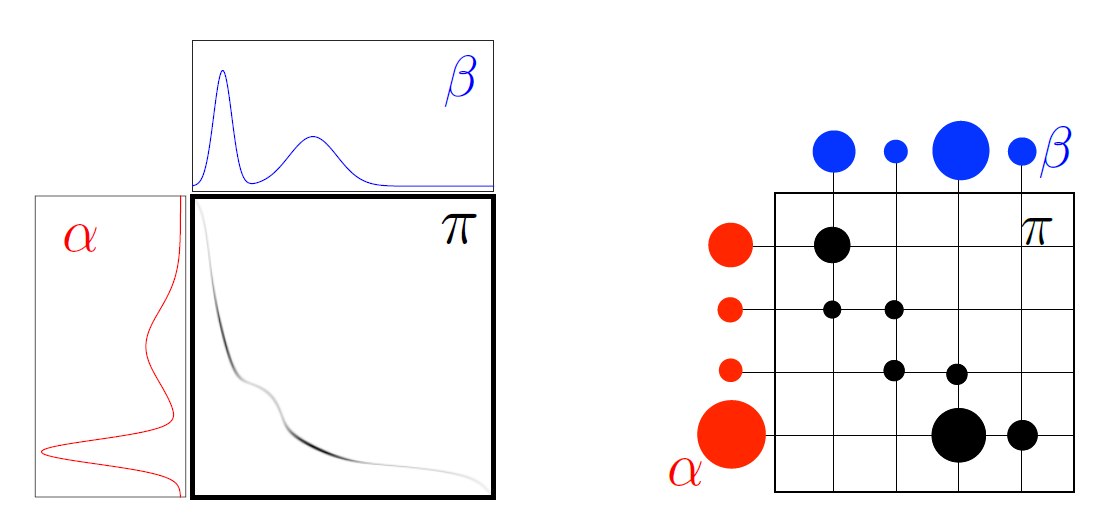
\includegraphics[width=0.7\textwidth]{img/transporte/coupling-example.png}
		  \caption{Izquierda: coupling óptimo entre dos medidas 1-D continuas con densidad. El coupling está localizado a lo largo del grafo del mapa de transporte óptimo $(x, T(x))$. Derecha: coupling óptimo entre dos medidas discretas. El radio del disco negro es proporcional a la masa transportada en esa coordenada. Imagen obtenida de \cite{peyre2019computational}.
			  \label{fig:coupling-example}}
	  \end{figure}

	  Y utilizando esta definición, se puede definir el problema de transporte óptimo de Kantorovich:
	  \begin{definition}[Problema de \cite{kantorovich1942translocation}]
		  Dadas dos medidas $\mu \in \ProbSpace[\cX]$ y $\nu \in \ProbSpace[\cY]$ y una función de coste $c: \cX \times \cY \to \R$, el \emph{problema de transporte óptimo de Kantorovich} se define como el problema de encontrar un coupling $\pi \in \Cpl(\mu, \nu)$ que minimice el costo total de transporte, es decir, que minimice la siguiente expresión:
		  \begin{equation}
			  \label{eq:problemaTransporteKantorovich}
			  \inf_{\pi \in \Cpl(\mu, \nu)} \int_{\cX \times \cY} c(x, y) \dpi[x, y] .
		  \end{equation}
		  Al conjunto de couplings que resuelven este problema se le llama \emph{planes de transporte} o \emph{couplings óptimos}, y se denotará por $\pi_{\mu \to \nu}$, o simplemente $\pi$ si es que no existe confusión.
	  \end{definition}


	  En diferencia con el problema de Monge, el problema de Kantorovich siempre tiene solución, si es que $(\cX, \cY)$ son espacios compactos y $c$ es continuo. En efecto, $\Cpl(\mu, \nu)$ es compacto para la topología débil de las medidas, $\pi \mapsto \int c\dd{\pi}$ es una función continua para esta topología, y la restricción $\pi\in\Cpl(\mu, \nu)$ es no vacía (la medida producto $\mu \otimes \nu$ pertenece a $\Cpl(\mu, \nu)$). Como se busca un ínfimo en un compacto de una función continua, se sigue que existe un coupling óptimo $\pi_{\mu \to \nu}$ que resuelve \eqref{eq:problemaTransporteKantorovich}.

	  %   Ejemplos de couplings óptimos se pueden apreciar en la Figura~\ref{fig:coupling-example}.

	  Continuando con los ejemplos \ref*{ex:problemaDeMongeSinSolucion} y \ref*{ex:problemaDeMongeMultipleSolucion}, podemos encontrar el coupling óptimo para cada uno de estos problemas:

	  \begin{example}
		  Sean los espacios $\cX$ y $\cY$ y las medidas $\mu$ y $\nu$ como en el Ejemplo~\ref*{ex:problemaDeMongeSinSolucion}. En este caso, el coupling óptimo entre $\mu$ y $\nu$ corresponde a:
		  \begin{align*}
			  \pi_{\mu \to \nu}\left\{ (-1, 0) \right\} & = \frac{1}{2} & \pi_{\mu \to \nu}\left\{ (1, 0) \right\} & = \frac{1}{2}.
		  \end{align*}
		  Del mismo modo, el coupling óptimo entre $\nu$ y $\mu$ corresponde a:
		  \begin{align*}
			  \pi_{\nu \to \mu}\left\{ (0, -1) \right\} & = \frac{1}{2} & \pi_{\nu \to \mu}\left\{ (0, 1) \right\} & = \frac{1}{2}.
		  \end{align*}

	  \end{example}

	  \begin{example}
		  Del mismo modo, Sean los espacios $\cX$ y $\cY$ y las medidas $\mu$ y $\nu$ como en el Ejemplo~\ref*{ex:problemaDeMongeMultipleSolucion}. En este caso, el coupling óptimo entre $\mu$ y $\nu$ corresponde a:
		  \begin{align*}
			  \pi_{\mu \to \nu}\left\{ ((1, 1), (-1, 1)) \right\}   & = \frac{1}{4} & \pi_{\mu \to \nu}\left\{ ((1, 1), (1, -1)) \right\}   & = \frac{1}{4}  \\
			  \pi_{\mu \to \nu}\left\{ ((-1, -1), (-1, 1)) \right\} & = \frac{1}{4} & \pi_{\mu \to \nu}\left\{ ((-1, -1), (1, -1)) \right\} & = \frac{1}{4}.
		  \end{align*}

	  \end{example}

	  Para finalizar esta sección, una pregunta que surge naturalmente es: ¿Cómo se relacionan los problemas de Monge y Kantorovich? ¿Si es que encuentro una solución para el problema de Kantorovich, esta estará relacionada de algún modo con el problema de Monge?
	  La respuesta la podemos encontrar en el teorema de Brenier:

	  \begin{theorem}[\cite{brenier1991polar}]
		  Sea $\cX = \cY = \R^d$, $c(x, y) = \|x - y\|^2$, $\mu\in \ProbSpace[\cX] $ y $\nu\in \ProbSpace[\cY] $. Si al menos una de las dos medidas (que s.p.g. supondremos que es $\mu$) tiene densidad con respecto a la medida de Lebesgue, entonces el plan de transporte óptimo $\pi$ es único y esta soportado en el grafo $(x, T(x))$ de un mapa de transporte óptimo $T:\cX \to \cY$. Esto significa que $\pi = \pf{(\id, T)}\mu$, y que cumple la siguiente ecuación:
		  \begin{equation}
			  \forall h \in \cC(\cX \times \cY),\quad \int_{\cX\times\cY}^{} h(x, y) \dpi[x, y] = \int_{\cX}^{} h(x, T(x)) \dmu[x].
		  \end{equation}
		  Más aún, el mapa de transporte óptimo $T$ está unicamente definido como el gradiente de una función convexa $\phi$, i.e. $T(x) = \grad \phi(x)$, donde $\phi$ es la única función convexa (salvo una constante aditiva) tal que $\pf{(\grad \phi)} \mu = \nu$.
	  \end{theorem}

	  \begin{proof}
		  Se puede encontrar una demostración de este teorema en \cite[p. 27]{peyre2019computational}
	  \end{proof}


  }

  \section{La Distancia y el Espacio de Wasserstein}\label{sec:la-distancia-y-el-espacio-de-Wasserstein}
  {
	  \FM{Incluir subsections para la distancia, espacio, y convergencia débil?}
	  Como se revisó en la sección anterior, cuando se considera el problema de Kantorovich, este problema usualmente tiene solución. Ahora bien, nos podemos pregunta: ¿Qué sucede si la función de coste se reemplaza con una distancia? ¿Qué propiedades surgirán? En esta sección se responderá a estas preguntas. Para ello, se empezará definiendo la distancia de Wasserstein, para luego revisar algunas de sus propiedades.
	  %   En esta sección se presentará que, al evaluar la expresión \eqref{eq:problemaTransporteKantorovich} del problema de Kantorovich para una función de coste con distancia, se obtiene una distancia entre medidas de probabilidad. Revisaremos algunas propiedades de esta distancia, para concluir que esta distancia metriza la convergencia débil entre medidas de probabilidad.

	  \begin{definition}[La distancia de Wasserstein]\label{def:distanciaWasserstein}
		  Sea $(\cX, \dist)$ un espacio Polaco y sea $p \geq 1$. Para dos medidas $\mu, \nu$ sobre $\cX$, la distancia de Wasserstein de orden $p$ entre $\mu$ y $\nu$ es definida por medio de la fórmula
		  \begin{equation}
			  \label{eq:distanciaWasserstein}
			  \Wasserstein[p]{\mu}{\nu}  \eqdef \left( \inf_{\gamma \in \Cpl(\mu, \nu)} \int_{\cX \times \cX} \dist(x, y)^{p} \dgamma[x, y] \right)^{\frac{1}{p}}.
		  \end{equation}

	  \end{definition}

	  \begin{example}
		  $\Wasserstein[p]{\delta_x}{\delta_y} = \dist(x, y)$. Notemos que en este ejemplo, se puede interpretar que la distancia de Wasserstein metriza el ``esfuerzo'' de llevar la masa del punto $x$ al punto $y$, como se comentó en los problemas de Kantorovich y de Monge.
	  \end{example}

	  Como el nombre de $W_p$ puede adelantar, esta es una distancia sobre medidas de probabilidad. Sin embargo, si esta es definida sobre todo el espacio $\ProbSpace[\cX]$, entonces puede tomar valores de $+\infty$, de forma que en estricto rigor, $W_p$ aún no puede ser considerada una distancia.
	  Para remediar este problema, se definirá un espacio de medidas de probabilidad en el que la distancia de Wasserstein tome valores finitos.

	  \begin{definition}[El espacio de Wasserstein]
		  Con los mismos supuestos que en la Definición \ref{def:distanciaWasserstein}, se define el espacio de Wasserstein de orden $p$ por medio de
		  \begin{equation}
			  \WassersteinSpace[p]{\cX} \eqdef \left\{
			  \mu \in \ProbSpace[\cX] \colon \int_{\cX} \dist(x, x_0)^{p} \dmu[x] < \infty
			  \right\},
		  \end{equation}
		  para algún punto fijo $x_0 \in \cX$. De esta forma, $W_p$ define una distancia (finita) sobre $\WassersteinSpace[p]{\cX}$.
	  \end{definition}

	  En palabras simples, el espacio de Wasserstein de orden $p$ es el conjunto de medidas de probabilidad en $\cX$ cuyo momento de orden $p$ es finito.\FM{Será necesario este último comentario?}

	  En \cite[p. 94]{villani2009optimal} se puede encontrar una demostración de que $\WassersteinSpace[p]{\cX}$ satisface con los tres axiomas de una distancia. Es más, se puede demostrar que $\WassersteinSpace[p]{\cX}$ puede heredar varias propiedades del espacio base $\cX$, como lo presenta el siguiente teorema:
	  \begin{theorem}[Topología del espacio de Wasserstein, \cite{villani2009optimal}]
		  \label{thm:espacioWassersteinEsMetrico}
		  Si $(\cX, \dist)$ es un espacio Polaco, entonces el espacio de Wasserstein $\WassersteinSpace[p]{\cX} $, metrizado por la distancia de Wasserstein $W_p$, es también un espacio Polaco.
	  \end{theorem}

	  \begin{proof}
		  Revisar la demostración del Teorema 6.18 en \cite[p. 105]{villani2009optimal}
	  \end{proof}

	  \FM[inline]{Desde aquí en adelante, creo que se puede mover a otras secciones, si es que se necesita}

	  \FM[inline]{Creo que esta línea no es del todo necesaria}
	  A partir de ahora, se asumirá que el espacio $\WassersteinSpace[p]{\cX} $ siempre estará equipado con su respectiva distancia $W_p$.

	  \FM[inline]{Esta observación no es tan necesaria para esta primera parte de preliminares}
	  \begin{remark}
		  A través de la desigualdad de Hölder, se puede demostrar que para $p \leq q$, se tiene que $\Wasserstein[p]{\mu}{\nu} \leq \Wasserstein[q]{\mu}{\nu}$, para toda $\mu, \nu \in \WassersteinSpace[p]{\cX}$. Y por tanto, las topologías inducidas por las distancias de Wasserstein se van encajonando.

		  En particular, la distancia de Wasserstein de orden 1, es la más débil de todas. Como norma general, la distancia $W_1$  es la más flexible y fácil de acotar, mientras que la distancia $W_2$ posee mejores propiedades geométricas, pero es más difícil de trabajar.
	  \end{remark}

	  \FM[inline]{Esta observación la moveré cuando pase a ver las WGANs}
	  Vista la distancia y el espacio de Wasserstein, se presentará una caracterización de convergencia en este espacio. Para ello, se definirá la convergencia débil entre medidas de probabilidad.

	  \begin{definition}[Convergencia Débil]
		  Sea $(\cX, \dist)$ un espacio Polaco y sea $p \geq 1$. Se dice que una sucesión de medidas de probabilidad $(\mu_n)_{n \in \N} \subset \WassersteinSpace[p]{\cX} $ converge débilmente a $\mu \in \WassersteinSpace[p]{\cX}$ si
		  \begin{equation}
			  \forall \phi \in \ContBoundedSpace[\cX], \quad \int_{\cX} \phi(x) \dd{\mu_n(x)} \to \int_{\cX} \phi(x) \dmu[x].
		  \end{equation}
		  y lo denotaremos por $\mu_n \wto \mu$.
	  \end{definition}

	  \begin{note}
		  Intuitivamente, que una sucesión de medidas de probabilidad converjan débilmente a una medida $\mu$ significa que es la forma ``más fácil'' que tiene la sucesión de converger a $\mu$.
	  \end{note}

	  \begin{theorem}[La Distancia de Wasserstein Metriza la Convergencia Débil]
		  Sea $(\cX, \dist)$ un espacio Polaco y sea $p \geq 1$. Entonces, la distancia de Wasserstein $W_p$  metriza la convergencia débil en $\WassersteinSpace[p]{\cX}$.
	  \end{theorem}

	  \begin{remark}
		  En otras palabras, si $(\mu_n)_{n\in\N}$ es una sucesión de medidas de probabilidad en $\WassersteinSpace[p]{\cX}$ y $\mu\in \WassersteinSpace[p]{\cX} $ otra medida, entonces $\mu_n \wto \mu$ si y sólo si $\Wasserstein[p]{\mu_n}{\mu} \to 0$.
	  \end{remark}

	  \begin{example}
		  Consideremos las siguientes distancias y divergencias entre medidas de probabilidad:
		  \begin{gather*}
			  \TV{\mu}{\nu} \eqdef \sup_{A \subseteq \cX} \abs{\mu(A) - \nu(A)}, \\
			  \KL{\mu}{\nu} \eqdef \int_{\cX} \log\left(\dv{\mu}{\nu}(x)\right) \dmu[x], \\
			  \JS{\mu}{\nu} \eqdef \KL{\mu}{\frac{\mu + \nu}{2}} + \KL{\nu}{\frac{\mu + \nu}{2}},
		  \end{gather*}
		  donde la primera es la distancia total variación, la segunda es la divergencia de Kullback-Leibler, y la tercera es la divergencia de Jensen-Shannon.

		  Si consideramos $\delta_\theta$ y $\delta_0$ medidas de Dirac centradas en $\theta$ y $0$ respectivamente, entonces se puede demostrar que
		  \begin{align*}
			  \Wasserstein[1]{\delta_\theta}{\delta_0} & = |\theta|                            &
			  \TV{\delta_\theta}{\delta_0}             & = \begin{cases}
				                                               1 & \text{si } \theta \neq 0 \\
				                                               0 & \text{si } \theta = 0
			                                               \end{cases}          \\
			  \KL{\delta_\theta}{\delta_0}             & = \begin{cases}
				                                               +\infty & \text{si } \theta \neq 0 \\
				                                               0       & \text{si } \theta = 0
			                                               \end{cases} &
			  \JS{\delta_\theta}{\delta_0}             & = \begin{cases}
				                                               \log(2) & \text{si } \theta \neq 0 \\
				                                               0       & \text{si } \theta = 0
			                                               \end{cases}
		  \end{align*}
		  Entonces, si tomamos $\theta = \frac{1}{n} $ y dejamos que $n \to \infty$, se tiene que $\Wasserstein[1]{\delta_\theta}{\delta_0} \to 0$, pero el resto de distancias y divergencias no convergen a 0.
		  Por tanto, se puede notar que la distancia de Wasserstein es la única que es capaz de distinguir entre medidas de probabilidad que no tienen soporte en el mismo punto, gracias a que metriza la convergencia débil.
	  \end{example}

  }  % end of sec. La Distancia y el Espacio de Wasserstein

  \section{El Baricentro de Wasserstein Bayesiano}\label{sec:el-baricentro-de-Wasserstein-Bayesiano}
  {
	  En esta sección se presentará el concepto de baricentro de Wasserstein, el cual es una generalización del concepto de promedio para medidas de probabilidad. Este concepto será clave para definir el baricentro de Wasserstein Bayesiano, el cual será el principal objeto de estudio de esta memoria. Para ello, se empezará revisando el concepto de media de Fréchet, para luego definir el baricentro de Wasserstein. La escritura de esta sección se basó en ejemplos de \cite{panaretos2020invitation} y definiciones de \cite{peyre2019computational}.

	  \subsection*{La Media de Fréchet}\label{ssec:la-media-de-Frechet}
	  {
		  %   En esta sección se revisará el concepto de media de Fréchet, el cual es una generalización de la noción de promedio para espacios métricos. Este concepto será clave para definir el baricentro de Wasserstein.
		  \begin{definition}[Funcional y Media de \cite{frechet1948elements}]
			  Sea $(\cX, \dist)$ un espacio Polaco. Sean $x_1, \ldots, x_n$ puntos en $\cX$ y sean $\gamma_1,\ldots,\gamma_n\in\R_+$ los pesos asociados a esos puntos. Para cada $p\in\cX$, se define el \emph{funcional de Fréchet} por
			  \begin{equation}
				  \label{eq:funcionalFrechet}
				  \Psi(p) \eqdef \sum_{i=1}^{n} \gamma_i \dist(p, x_i)^2.
			  \end{equation}
			  Y, en caso de que exista un punto $m \in \cX$ que minimice el funcional $\Psi$, entonces este se definirá como la \emph{media de Fréchet} de los puntos $x_1,\ldots, x_n$. Es decir, es aquel punto tal que minimiza el siguiente problema:
			  \begin{equation}
				  \label{eq:mediaFrechet}
				  m \eqdef \argmin_{p \in \cX} \sum_{i=0}^{n} \gamma_i \dist(p, x_i)^2.
			  \end{equation}
		  \end{definition}

		  \begin{example}\label{ex:baricentro-triangulo}
			  Tomemos $x_1, x_2, x_3 \in \R^2$ tres puntos en el plano, formando un triángulo. Si se define el promedio (o el \textit{baricentro}, en el contexto de la geometría) de estos puntos por $\bar x = \frac{1}{3} (x_1 + x_2 + x_3)$, entonces se puede comprobar fácilmente que este es el único que minimiza el funcional de Fréchet:
			  \begin{equation}
				  F(p) = \frac{1}{3} \sum_{i=0}^{3} \|p - x_i\|^2,
			  \end{equation}
			  puesto que este funcional se puede descomponer de la siguiente manera:
			  \begin{equation}
				  F(p) = F(\bar x) + \|p-\bar x\|^2.
			  \end{equation}
			  Con este ejemplo, se puede apreciar que la media de Fréchet generaliza la noción de promedio.
		  \end{example}

		  \begin{remark}
			  La razón por la que resulta interesante estudiar este concepto, es que únicamente utiliza nociones métricas, desligándose de nociones vectoriales. Como se vió en el Ejemplo~\ref{ex:baricentro-triangulo}, el promedio $\bar x$ utilizó conceptos vectoriales (suma y ponderación de vectores) mientras que la media de Fréchet utilizó nociones métricas, resultando en el mismo promedio.

			  Aunque igualmente se hizo algo de ``trampa'', pues se utilizó la norma para definir una distancia. Sin embargo, el concepto es mucho más general, pues este baricentro depende de la distancia que se esté utilizando, de forma que el baricentro cambiará conforme a esta.
		  \end{remark}

	  }  % end of sec. La Media de Fréchet

	  \subsection*{El Baricentro de Wasserstein}\label{ssec:el-baricentro-de-Wasserstein}
	  {
		  Como se vió en la sección anterior, la media de Fréchet permite definir una noción de promedio para espacios métricos. Como se vió en la sección anterior, el Teorema~\ref{thm:espacioWassersteinEsMetrico} establece que $(\WassersteinSpace[p]{\cX}, W_p)$ es un espacio métrico, y por tanto, se puede definir su respectivo ``promedio'':

		  \begin{definition}[Baricentro de Wasserstein, \cite{agueh2011barycenters}]
			  Sean $\mu_1,\ldots, \mu_n \in \WassersteinSpace[p]{\cX} $ y sean $\gamma_1,\ldots, \gamma_n \in \R_+$ sus pesos asociados. El \emph{baricentro de Wasserstein} se define por medio de
			  \begin{equation}
				  \bar \mu \eqdef \arginf_{\nu \in \WassersteinSpace[p]{\cX} } \sum_{i=0}^{n} \gamma_i \Wasserstein[p]{\nu}{\mu_i}^p
			  \end{equation}

		  \end{definition}
		  \FM[inline]{Se podría poner algún ejemplo con una imagen.}

		  Es posible generalizar aún más la noción de baricentro de Wasserstein a una colección infinita de medidas. Esto se puede hacer considerando una medida $\Gamma \in \ProbSpace[\ProbSpace ] $, que cumplirá el rol de los pesos $\gamma_1,\ldots, \gamma_n $ en la definición anterior. Esto se puede formalizar en la siguiente definición:

		  \begin{definition}[Baricentro de Wasserstein, versión general]
			  Sea $\Gamma \in \ProbSpace[\ProbSpace]$ una medida. El baricentro de Wasserstein se puede (re)-definir como aquel que minimice el siguiente problema:
			  \begin{equation}
				  \bar \mu \eqdef \arginf_{\mu \in \ProbSpace} \int_{\ProbSpace} \Wasserstein[p]{\mu}{\nu}^p \dd{\Gamma(\nu)}
			  \end{equation}

		  \end{definition}

		  \begin{remark}
			  Se puede notar que la definición anterior es una generalización, pues si se considera $\Gamma = \sum_{i=1}^{n} \gamma_i \delta_{\mu_i}$, entonces se recupera la primera definición.
		  \end{remark}



	  }  % end of sec. El Baricentro de Wasserstein


	  \subsection{Geodésicas en el Espacio de Wasserstein}\label{ssec:geodesicas-Wasserstein}
	  {
		  En esta sección, se utilizará la distancia de Wasserstein para definir una noción de geodésica en el espacio de Wasserstein. Esta noción será de utilidad para definir el baricentro de Wasserstein Bayesiano.
		  \FM[inline]{Agregar la referencia del Lecture}
		  \FM{Podría agregar la imagen de geodésica de la presentación de Cuturi}
		  \begin{definition}
			  Sea $(\cX, \dist)$ un espacio métrico. Una \emph{geodésica a velocidad constante}  entre dos puntos, $x_0, x_1 \in \cX$ es una curva continua $x : [0, 1] \to \cX$  tal que para cada $s, t \in [0, 1]$, $\dist(x_s,x_t) = |s - t| \dist(x_0,x_1) $.\FM{Debería de quitar esta definición? Nunca la ocupo directamente.}
		  \end{definition}

		  \begin{proposition}
			  Sean $\mu_0, \mu_1 \in \WassersteinSpace[p]{\cX} $, con $\cX \in \R^d$  compacto y convexo. Sea $\gamma \in \Cpl(\mu_0, \mu_1)$  un plan de transporte óptimo\FM{Agregar en la def que estos se llamarán planes de transporte}. Definamos
			  \begin{equation}
				  \mu_t \eqdef \pf{(\pi_t)} \gamma, \quad \text{donde } \pi_t(x, y) = (1-t)x + ty.
			  \end{equation}
			  Entonces, la curva $\mu_t$ es una geodésica a velocidad constante entre $\mu_0$ y $\mu_1$.

		  \end{proposition}

		  \begin{example}
			  Si existe un mapa de transporte óptimo $T$ entre $\mu_0$ y $\mu_1$, entonces la geodésica definida arriba es $\mu_t = \pf{((1-t)\id + tT)} \mu_0$.
		  \end{example}

		  \FM[inline]{Creo que esta observación no es tan importante por ahora}
		  \begin{remark}
			  En caso en que $\mu_0 = \sum_{i=1}^{n} m_i \delta_{x_i}$ y $\mu_1 = \sum_{i=1}^{n} m_i \delta_{y_i}$, con $m\in\Simplex[n]$ y $x_1,\ldots, x_n, y_1,\ldots, y_n \in \cX$, entonces la geodésica definida arriba se puede escribir de la siguiente manera:
			  \begin{equation}
				  \mu_t = \sum_{i=1}^{n} m_i \delta_{(1-t)x_i + ty_i},
			  \end{equation}
			  lo que se puede interpretar como que la masa $m_i$ del punto $x_i$ se transporta al punto $y_i$ a velocidad constante.
		  \end{remark}




	  }  % end of sec. Geodésicas en el Espacio de Wasserstein

	  \subsection{El Baricentro de Wasserstein Bayesiano}\label{ssec:baricentro-Wasserstein-Bayesiano}
	  {
		  En esta sección se definirá el baricentro de Wasserstein Bayesiano, el cual es una generalización del baricentro de Wasserstein, que permite incorporar información a priori sobre las medidas de probabilidad que se quieren promediar. En esta sección se utilizará como referencia principal \cite{rios2020contributions} y \cite{backhoff2022bayesian}.

		  Se considerarán muestras $\Data = \left(x_1,\ldots, x_n \right)$ en un espacio $\cX$ y un conjunto de modelos factibles, o medidas de probabilidad $\Models \subseteq \ProbSpace[\cX]$. Aprender un modelo, también conocido como la \emph{selección de un modelo}, utilizando los datos $\Data$ consiste en escoger un elemento $\mu$ de $\Models$ que mejor explique los datos, si es que estos hubieran sido generados por $\mu$.

		  Para ello, se adoptará un enfoque Bayesiano, el cuál provee de un marco probabilística para manejar la incertidumbre sobre los modelos. Por tanto, se empezará considerando una medida de probabilidad $\Pi \in \ProbSpace[\ProbSpace[\cX] ] $, entendida con una distribución a \textit{priori} sobre un espacio de modelos $\Models$. En particular, se tiene que el prior se encuentra soportada en el espacio de modelos $\Models$, es decir, $\Pi(\Models) = \Pi(\ProbSpaceAC[\cX] ) = 1$.

		  Para cada $n \in \N\setminus\left\{ 0 \right\}$, $\Pi$ induce una ley canónica $\bPi$ sobre $\cX^n\times \Models$, representando una ley conjunta de un modelo $\mu$ escogida de acuerdo a $\Pi$ y una muestra i.i.d $\Data = (x_1,\ldots, x_n) \in \cX^n$ generada por $\mu$. Esto es
		  \begin{equation}
			  \dd{\bPi(x_1,\ldots, x_n, \mu)}
			  \eqdef \dd{\Pi(\mu)} \dd{\mu(x_1)} \cdots \dd{\mu(x_n)}
			  = \dd{\Pi(\mu)} \dd{\lambda(x_1)} \cdots \dd{\lambda(x_n)} \prod_{i=1}^{n} \dv{\mu}{\lambda} \qty(x_i),
		  \end{equation}
		  donde $\dv{\mu}{\lambda}$ denota la derivada de Radon-Nikodym de $\mu$ con respecto a $\lambda$. Considerando que $\dd{\bPi(x_1,\ldots, x_n, \mu)} = \bPi(\dd x_1,\ldots, \dd x_n \mid \mu) \dd{\Pi(\mu)}$, la ley sobre $\cX^n$ de los datos $\Data$, condicional al modelo $\mu$, está dado por
		  \begin{equation}
			  \dd{\bPi(x_1,\ldots, x_n, \mu)}
			  \eqdef \prod_{i=1}^{n} \dv{\mu}{\lambda} \qty(x_i)  \dd{\lambda(x_1)} \cdots \dd{\lambda(x_n)} \dd\Pi(\mu),
		  \end{equation}
		  donde la densidad marginal de $\Data$ con respecto a $\lambda^{\otimes n}$ es
		  \begin{equation*}
			  \dv{\bPi}{\lambda^{\otimes n}}\qty(x_1,\ldots, x_n) = \int_{\Models} \prod_{i=1}^{n} \dv{\nu}{\lambda}\qty(x_1) \dd{\Pi(\nu)}.
		  \end{equation*}

		  La \textit{distribución posterior} $\bPi(\dd \mu \mid x_1, \ldots, x_n )$ dada la data $\Data$ es también un elemento de $\ProbSpace[\ProbSpace[\cX] ] $, el cuál se denotará por $\Pi_n$ por simplicidad y el cuál, en virtud a la regla de Bayes, está dado por
		  \begin{equation}
			  \label{eq:distribucionPosterior}
			  \dd{\Pi_n(\mu)}
			  \eqdef \frac{\bPi(x_1,\ldots, x_n \mid\mu)}{\bPi(x_1,\ldots, x_n)} \dd{\Pi(\mu)}
			  = \frac{\prod_{i=1}^{n} \dv{\mu}{\lambda}\qty(x_i)}
			  {\int_{\Models} \prod_{i=1}^{n} \dv{\nu}{\lambda}\qty(x_1) \dd{\Pi(\nu)}} \dd{\Pi(\mu)}.
		  \end{equation}





		  %   de tamaño $n$ generada por $\mu$. En particular, se tiene que $\bPi$ es una medida de probabilidad sobre $\cX^n\times \Models$ tal que

		  %   \FM[inline]{Comentar que aquí se está tomando ideas de la tesis de Gonzalo Ríos}
		  %   Consideremos muestras $\Data = \left\{ x_1,\ldots, x_n  \right\}$ en un espacio $\cX$ y un conjunto de modelos factibles o medidas de probabilidad $\Models \subseteq \ProbSpace[\cX]$. Aprender un modelo, también conocido como la \emph{selección de un modelo}, de $\Data$ consiste en escoger un elemento $\mu \in \Models$ que mejor explique los datos, si es que estos hubieran sido generados por $\mu$, dado algún criterio.

		  %   Se considerará una medida de probabilidad $\Prior \in \ProbSpace[\Models]$ sobre un espacio de modelos $\Models$  un \emph{prior} fijo.
	  }  % end of sec. El Baricentro de Wasserstein Bayesiano

  }  % end of sec. El Baricentro de Wasserstein


  \FM[inline]{Será necesario incluir una parte que describa métodos numéricos para calcular baricentros? Tenía pensado incluir el algoritmo del descenso del gradiente estocástico en espacio de Wasserstein, los algoritmos LP para el problema de Wasserstein, el de Sinkhorn, el Convolucional y el Debaised, que igual fueron métodos estudiados y utilizados.}
 }